\documentclass[uplatex,dvipdfmx,a4paper,twocolumn,base=11pt,jbase=11pt,ja=standard]{bxjsarticle}  % 環境に合わせて変更してください

\usepackage{ipsj}
\usepackage{color}

%追加パッケージ
\usepackage{enumerate}
\usepackage{url}
\usepackage[dvipdfmx]{graphicx}
\usepackage{caption}

\newcommand{\todo}[1]{\colorbox{yellow}{{\bf TODO}:}{\color{red} {\textbf{[#1]}}}}

\title{直観的なScratch作品のためのユーザ入力タイミング特定の試み}{Toward identifying user input timing for intuitive Scratch work search}
\author{和歌山大学}{岡本 圭悟}{Keigo Okamoto, Wakayama University}
\author{和歌山大学}{伊原 彰紀}{Akinori Ihara, Wakayama University}
\author{和歌山大学}{三倉 舞子}{Maiko Mikura, Wakayama University}
\author{和歌山大学}{橋谷 直樹}{Naoki Hashitani, Wakayama University}

\begin{document}
\maketitle


%================
%1
\section{はじめに}
%================

%最後に言っていることを統一する
%結果にどのような作品が取れるようになることを期待しているのかを記述する
%はじめにでこんなことをすると,全体的なことを言っておいて手法では今回はこんなことだけやると言ったことを書く.
%(今後は量を集計することは言いつつ,今回はスナップショットの撮影だけという.)
%
%ビジュアルプログラミング言語の学習環境であるScratch\footnote{\url{Scratch: https://scratch.mit.edu/}}では,ユーザはキーワード検索によって他者が制作した作品を参照し,多様な実装方法を学習できる.


ビジュアルプログラミング言語の学習環境の一つであるScratch\footnote{\url{Scratch: https://scratch.mit.edu/}}では,多様な実装方法を学習/参照するために膨大な作品が公開されており,キーワード検索によって絞り込む機能を有する.
%検索できる.でもXXは検索できない.
しかし,ユーザが実装したい動作イメージを言語化することは容易でないため,そのイメージに類似する作品の検索は困難である.
%イメージの実装に適した作品を検索することは困難である.
従来研究\cite{thesis_fukuchi2021}では,ユーザがイメージするオブジェクトの移動軌跡をマウス操作によって入力し,それをクエリとしてイメージに類似する作品検索を実現しているが,検索にはあらかじめ作品を自動実行してスナップショットを撮影する必要があるため,入力操作を持つ作品は対象にできていない.

本研究の事前分析ではScratchの入力操作を持つ作品数,および実装に必要な計算論理的思考能力をDr.Scratch~\cite{RED2015_J. Moreno-Le ́on}を用いて定量的に計測した.Scratchの入力操作を持つ作品は,入力操作を持たない作品の10倍以上存在する.また,図1は入力操作を持つ作品と入力操作を持たない作品の実装に必要な計算論理的思考のスコア[0-21]の分布を示す.マンホイットニーのU検定より,データ間に有意差があることも示された.このことから,入力操作を持つ作品はより多様な命令処理を必要とすることは明らかである.したがって,入力操作を有する作品を検索の対象に含むべきであるが,入力のタイミングをオブジェクトの移動軌跡のみから判断することは容易でない.

%Scratch作品中のオブジェクトの移動軌跡を用いた動作イメージを入力とする作品検索を実現した.実行画面上の画像オブジェクトの移動の軌跡を取得する際には作品を自動実行してスナップショットを撮影する必要があるため,ユーザの入力操作を有する作品は入力操作を行うタイミングが不明であり検索の対象外であった.

%事前分析より,ユーザの入力操作を有する作品は有さない作品の10倍以上存在し,Dr.Scratch~\cite{RED2015_J. Moreno-Le ́on}で測定できるコンピュテーショナル・シンキングスコアの平均値が高いことが明らかとなった.\todo{マンホイットニーU検定使えばすぐ.後にないならちゃんと書くべき.数値で.}

本論文では,入力を有する作品検索に向けて,作品中でユーザが入力操作するタイミングを特定し,自動実行するシステムを提案する.
%キー入力に注目し,作品を自動実行してスナップショットを撮影する際に自動で入力操作を行うタイミングを特定する.
具体的には,Scratchプログラムから,入力前後の命令処理,入力内容,入力前後のオブジェクトの位置を収集し,ユーザが入力操作するタイミングを特定する.

\begin{figure}
\begin{center}
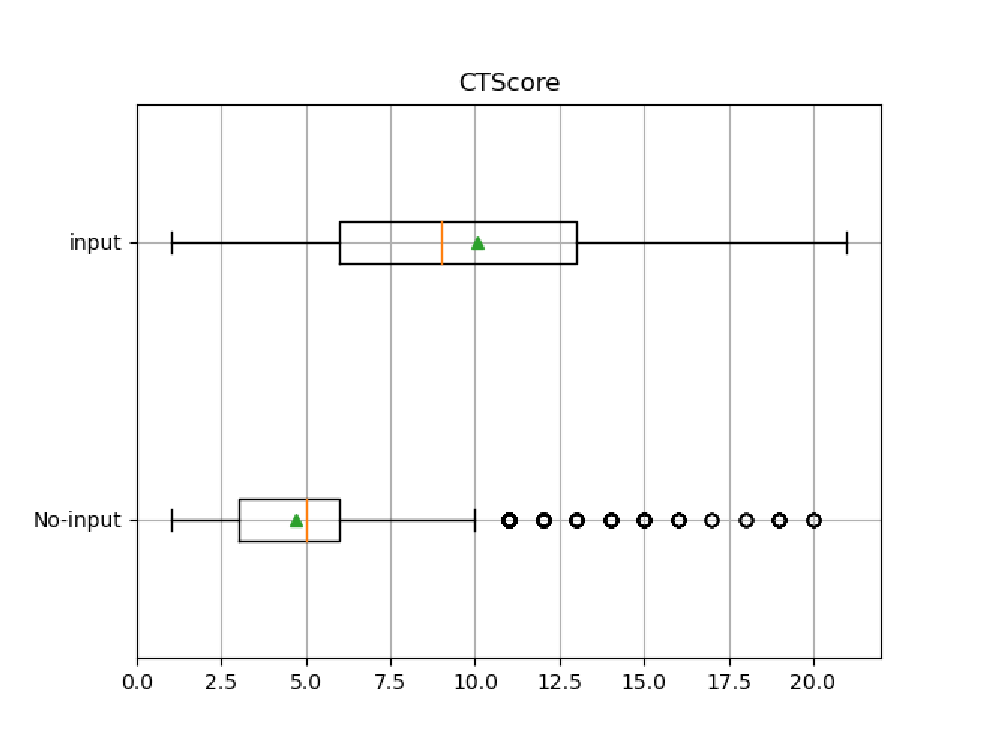
\includegraphics[width=0.9\linewidth]{plot.eps}
\caption{入力操作をもつ作品と持たない作品のCTスコアの分布}
\label{fig:test}
\end{center}
\end{figure}

%を解析して取得した「ユーザの操作を有するブロック」,「座標移動を行うブロック」,「ブロックの実行順序」の情報から,プログラム上で座標移動情報を計算し,実行画面上の画像オブジェクトの座標移動情報と照合することで入力すべきタイミングの特定を行う.


%================
%2
\section{実験}
%================


%2.1
\subsection{データセット}
%================
%hogehoge(どんなデータセット使ったか)

%fugofugo(そこからどんなデータをどうやって集めたか)
%npmエコシステムから収集した4hoge2のリポジトリからランダムに1000リポジトリ選択し,最新のREADMEを取得.READMEの中で見出しが使用法に分類されるものを抽出した.使用法にカテゴライズされたのは1000のREADMEの内,「usag(452件)」「exampl(119件)」「use(98件)」「method(10件)」...と「metod」以降は数が少ないため,本論文では上位3件である「usag」「exampl」「use」を使用する.

%2.1の修正版

本論文では,Scratch上で公開されている作品から,以下に示す条件を満たす作品を用いる.
\begin{itemize}
 \item ユーザの操作を有するブロックのうち,文字の入力でないキー入力のみを有するブロックを含む作品
 \item スクリプトが一つである作品
 \item 座標移動を行うブロックを含む作品
 \item Scratchが標準画像として用意する画像を含む作品
\end{itemize}


%npmエコシステムから収集した\todo{4hoge2}のリポジトリからランダムに1,000リポジトリを選択し,最新のREADMEファイルを取得する.取得したREADMEファイルの中から,本論文ではケーススタディとして「使用法」の項目に分類される部分を抽出した.使用法という項目について書かれているものは1000のREADMEの内,「usag(452件)」「exampl(119件)」「use(98件)」「method(10件)」...がある.「metod」以降は数が少ないため,上位3件である「usag」「exampl」「use」を使用する.例として「usag」には「Usage」や「usages」などの見出し語が含まれており,同一の見出し語「usag」として扱う.


%================
%2.2
\subsection{提案手法}
%================

%2.2の修正版


\noindent\textbf{1. XX: }対象のScratch作品に含まれる座標ブロック,ユーザの操作を有するブロック,ブロックの実行順序の情報を予め取得しておく.\\
\noindent\textbf{2. XX: }取得した情報を用いて,作品が実行されてからユーザの操作を有するブロックが処理されるまでにオブジェクトが到達する座標をプログラム上で計算する.\\
\noindent\textbf{3. XX: }作品実行時に2で得た座標に画像オブジェクトが到達したときを入力すべきタイミングとして,自動でキーを押下する.これをスクリプトが処理を終了するまで繰り返す.

「ループブロック」などの制御ブロックはその中の処理が終了したことをスクリプトの処理の終了として扱う.また,並列にスクリプトが存在する場合も同様の手順でスナップショットを撮影する.
%また,Scratchでは「キーが押された時ブロック」などのイベントブロックを複数持ちいるとスクリプトを並列に配置することができ,その実行タイミングや順序はユーザの意志に委ねられる.そのため,本手法では最初に実行される「実行ボタンが押された時ブロック」が含まれたスクリプトが終了した時,並列に他のスクリプトが存在する場合はスクリプトの数の通りだけスクリプトを実行して,それぞれでスナップショットを撮影することとする.
%\todo{サブルーチンも撮影しますって書くだけ}
%また,並列にスクリプトが存在する作品についても同様の方法で.
%また,Scratchでは「キーが押された時ブロック」などのイベントブロックを複数持ちいるとスクリプトを並列に配置することができ,その実行タイミングや順序はユーザの意志に委ねられる.そのため,本手法では最初に実行される「実行ボタンが押された時ブロック」が含まれたスクリプトが終了した時,並列に他のスクリプトが存在する場合はスクリプトの数の通りだけスクリプトを実行して,それぞれでスナップショットを撮影することとする.\todo{サブルーチンも撮影しますって書くだけ}


%================
%2.4
\subsection{ケーススタディ}
%================
%https://ja.overleaf.com/project/63bed14612a4c046c3cc848f/detacher
\noindent\textbf{[概要]}本手法で撮影したスナップショットと従来研究で撮影したスナップショットを比べ,どのような動作やブロックを持つ作品が検索の対象になり得るのかを調査する.

\noindent\textbf{[結果]}\todo{結果:従来研究のスナップショットと本手法で撮影したスナップショットを比べて実際にどのような作品が撮影できるようになったのかを記述します}


%--------------------------------
%2.4の修正版






%================
%3
\section{おわりに}
%================

%hogehoge(今回の研究のまとめとか)

%fugofugo(今回研究から得られたことを踏まえて今後どう発展させていくか)

%42(どんな研究をしていくつもりなのか的な)
%今回の研究のから hogehoge-fugofugoである.

%今後の展望として,本論文ではnpmエコシステムからデータを利用したが,他のエコシステムからのデータでも同様に分析を行い,結果を比較する.また,SVM以外の手法との結果も比較することを考えている.最終的な目標として,READMEに書くべき見出し語の自動生成や推薦を目標にしたいと考えている.

%本論文は,READMEにおける見出し,特に利用頻度の高い「利用方法」の見出しと見出し後の説明文の一貫性をSVMモデルを用いて分析した.\todo{XXがわかった.}今後は,利用方法に限らず,RAEDMEの説明文に基づく見出しの統一化に向けた分析を行う.

%今回の分析の結果から「使用法」という項目について書かれた内容から見出し語の予測をすることは現段階では難しいということが分かった.しかし,今回は内容に明確な違いがあるのかを示すことが目的であり,大きな差がないということがわかったため今後の展望として,「tf-idf」や「ランダムフォレスト」を用いることで,表記揺れが起きる見出し語間に見出し語を決める決定的な単語があるのかを調査したいと考える.また,今回は「使用法」を選択したが他の項目での結果を確かめるとともにデータ数を増やす必要があると考える.


%本論文は,READMEにおける見出し,特に利用頻度の高い「使用方法」の見出しと見出し語の説明文の一貫性をSVMモデルを用いて分析した.分析の結果,開発者はusag,example, useの見出し語を区別せずに使用していると考えられる.今後は,開発者の効率的なREADME作成および利用者のスムーズなREADME閲覧のために,使用方法に限らず,見出し語の説明文に基づく見出し語の統一に向け分析を行い,READMEファイルのガイドラインの作成に取り組む.
%本論文は,README における見出し,特に利用頻度の高い「使用方法」の見出しと見出しの説明文の一貫性を SVM モデルを用いて分析した.分析の結果,開発者は usag,example, use の見出しを区別せずに使用していると考えられる.今後は,READMEの説明文に対応する統一した見出しを分析し,README を作成するためのガイドラインの確立を目指す.


本論文では,入力を有する作品を含んだ学習者の動作イメージと類似する作品検索に向けて.自動で入力操作を行うタイミングの特定を試みた.今後の方針として,本手法を用いて撮影したスナップショットを用いて実際にどれだけ検索候補の数が向上したかどうかを確かめる.
%今後は,使用方法に限らず,READMEファイルの説明文に基づく見出しのガイドライン作成に向けた分析を行う.\todo{今後は...のところは石岡君の気持ちを込めた文章,に書き換えてください.}

%見出し語の説明文から見出し語を予測することが可能であると示唆されるが,見出し語と見出し語の説明文に一貫性がないものがあると考えられる.
%今後は,使用方法に限らず,READMEファイルの説明文に基づく見出しのガイドライン作成に向けた分析を行う.



%3の修正版







%================
\section*{謝辞}
%================

\todo{謝辞}

\begin{thebibliography}{1}
  \bibitem{thesis_fukuchi2021} 福地ユキ,伊原彰紀,山本豪志朗,橋谷直樹,オブジェクトの動作に基づくScratch作品の直感的検索手法,\todo{会議名}, 2021
  \bibitem{RED2015_J. Moreno-Le ́on} J. Moreno-Le'on, G. Robles, and M. Rom'an-Gonz'alez, ``Dr. scratch: Automatic analysis of scratch projects to assess and foster computational thinking,'' RED.Revista de Educaci'on a Distancia, vol.15, no.46, pp.1-23, 2015.
  \bibitem{ICMSR2017_Aivaloglou} E. Aivaloglou, F. Hermans, J. Moreno-Le'on, Gr. Robles, ``A dataset of scratch programs: scraped, shaped and scored,'' Proceeding of the International Conference on Mining Software Repositories (MSR'17), pp.511-514, 2017. 

\end{thebibliography}




\bibliographystyle{ipsjunsrt}
%\bibliography{bibfile}

\end{document}
